\usetikzlibrary{arrows.meta,shapes.symbols,shapes.multipart}

\begin{frame}{mailbox model: importance of naming}
    \begin{itemize}
    \item \textit{mailbox} abstraction: send/receive messages
    \end{itemize}
    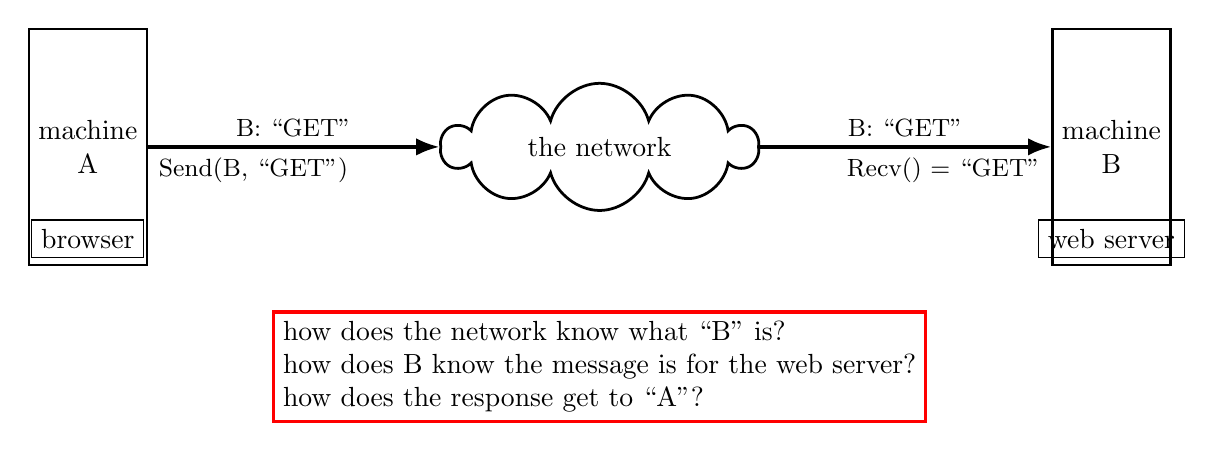
\begin{tikzpicture}
    \tikzset{
        >=Latex,
        comp box/.style={draw, thick, align=center, minimum width=1.5cm,minimum height=3cm},
        explain box/.style={draw=red,very thick, align=left},
        msg/.style={font=\small},
        cmd/.style={font=\small},
    }
        \node[comp box] (machine A) at (-6.5, 0) {machine \\ A};
        \node[draw,cloud,line width=1pt,minimum width=4cm,minimum height=1cm,aspect=3,
                ] (network) at (0,0) {the network};
        \node[comp box] (machine B) at (6.5, 0) {machine \\ B};
        \draw[very thick,->] (machine A) -- (network)
            node[midway,above,msg] {B: ``GET''}
            node[pos=0.0,below right,cmd] {Send(B, ``GET'')};
        \draw[very thick,<-] (machine B) -- (network)
            node[midway,above,msg] {B: ``GET''}
            node[pos=0.0,below left,cmd] {Recv() = ``GET''};
        % FIXME: hilite network: knows how to get message to particular place
            % note/show buffering at A/B


        \node[anchor=south,draw,rectangle,] at ([yshift=.1cm]machine A.south) {
            browser
        };
        \node[explain box,anchor=north] at ([yshift=-1.25cm]network.south) {
            how does the network know what ``B'' is? \\
            how does B know the message is for the web server? \\
            how does the response get to ``A''?
        };
        \node[anchor=south,draw,rectangle,] at ([yshift=.1cm]machine B.south) {
            web server
        };
    \end{tikzpicture}
\end{frame}